\documentclass[border=1mm]{standalone}

\usepackage{listings}
\usepackage{tikz}
\usetikzlibrary{positioning,fit,calc}
\usetikzlibrary{shapes.multipart}
\pgfsetlayers{background,cpu,main}

\pgfdeclarelayer{background}
\pgfdeclarelayer{cpu}
\pgfdeclarelayer{main}

\newsavebox\mybox

\lstset{language=Python}


\begin{document}

\begin{lrbox}{\mybox}
\begin{lstlisting}
      a = 5
      for i in range(a):
          b = a*(a-1)
          print( b )
      print( "ferdig!" )
\end{lstlisting}
\end{lrbox}


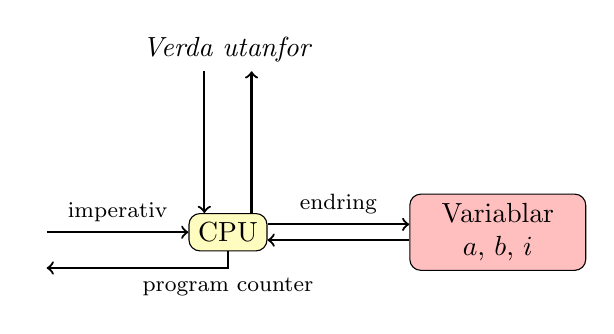
\begin{tikzpicture}[
  node distance=18mm,
  title/.style={font=\fontsize{6}{6}\color{black!50}\ttfamily}
  ]

   \node (prg) { \usebox\mybox } ;

   \node (cpu) [draw,rounded corners,fill=yellow!25,right=of prg] { CPU } ;
   \node (var) [draw,rounded corners,fill=red!25,right=of cpu] { \parbox{20mm}{\centering Variablar\\ $a$, $b$, $i$} } ;
   \draw [thick, ->] (prg) to node[above] {\footnotesize imperativ} (cpu);
   \draw [thick, ->] ([yshift=1mm]cpu.east) to node[above] {\footnotesize endring} ([yshift=1mm]var.west);
   \draw [thick, <-] ([yshift=-1mm]cpu.east) to ([yshift=-1mm]var.west);

   \node (wrl) [above=of cpu] {\emph{Verda utanfor} } ;
   \draw [thick, <-] ([xshift=-3mm]cpu.north) to ([xshift=-3mm]wrl.south);
   \draw [thick, ->] ([xshift=3mm]cpu.north) to ([xshift=3mm]wrl.south);

   \draw [thick, ->] (cpu.south) |- node[below] {\footnotesize program counter} ([yshift=-3ex]prg.east);


\end{tikzpicture}
\end{document}

